\documentclass{article}

% Language setting 
% Replace `english' with e.g. `spanish' to change the document language
\usepackage[english]{babel}
\usepackage{xspace}
\usepackage{siunitx}

% Set page size and margins
% Replace `letterpaper' with `a4paper' for UK/EU standard size
\usepackage[letterpaper,top=2cm,bottom=2cm,left=3cm,right=3cm,marginparwidth=1.75cm]{geometry}

% Useful packages 
\usepackage{amsmath}
\usepackage{graphicx}
\usepackage{bookmark}
\usepackage[acronym]{glossaries}
%\usepackage[colorlinks=true, allcolors=blue]{hyperref}

\usepackage{spverbatim}
\usepackage{pifont}
\usepackage[dvipsnames]{xcolor}
\usepackage{pdfpages}
\usepackage[export]{adjustbox}

\newcommand{\reff}[1]{(\ref{#1})}

\newcommand{\RISCV}{\textbf{\gls{RISCV}}\xspace}
\newcommand{\ISA}{\texttt{\acrshort{isa}}\xspace}

\newcommand{\sort}{\texttt{\gls{bubble_sort}}\xspace}

\newcommand{\PC}{\textbf{\acrshort{pc}}\xspace}
\newcommand{\RAM}{\textbf{\acrshort{ram}}\xspace}
\newcommand{\ROM}{\textbf{\acrshort{rom}}\xspace}
\newcommand{\ALU}{\textbf{\acrshort{alu}}\xspace}

\newcommand{\cmark}{\color{OliveGreen}\ding{51}}%
\newcommand{\xmark}{\color{Red}\ding{55}}%


\makeglossaries
\newglossaryentry{RISCV}
{
    name=RISCV,
    description={\href{https://riscv.org/about/}{RISC-V} is an open standard \ISA}
}

\newglossaryentry{bubble_sort}
{
    name=bubble sort,
    description={Sometimes referred to as sinking sort, is a simple sorting algorithm that repeatedly steps through the input list element by element, comparing the current element with the one after it, swapping their values if needed \cite{wiki:bubble}}
}

\newglossaryentry{clk}
{
    name=clock cycle,
    description={Also known as a machine cycle or a clock tick, is the basic unit of time in a computer's \acrshort{cpu} and synchronous electronic}
}

\newglossaryentry{stall}
{
    name=stall,
    description={In the design of pipelined computer processors, a pipeline stall is a delay in execution of an instruction in order to resolve a \gls{hazard} \cite{wiki:stall}}
}

\newglossaryentry{hazard}
{
    name=hazard,
    description={In the domain of \acrfull{cpu} design, hazards are problems with the instruction pipeline in \acrshort{cpu} microarchitectures when the next instruction cannot execute in the following \gls{clk}, and can potentially lead to incorrect computation results. Three common types of hazards are data hazards, structural hazards, and control hazards (branching hazards) \cite{wiki:haz}}
}

\newglossaryentry{linking}
{
    name=linking,
    description={The act of 'linking' intended as the action on the code performed by the \gls{linker}}
}
\newglossaryentry{linker}
{
    name=linker,
    description={In computing, a linker or link editor is a computer system program that takes one or more object files (generated by a compiler or an assembler) and combines them into a single executable file, library file, or another "object" file
    \cite{wiki:link}}
}
\newglossaryentry{control_sig}
{
    name=control signal,
    description={In a \acrshort{cpu} is a signal that select the path of the data in the different stages of execution of the instruction. They determine for example the operations performed by the different components and the selection of the \acrshort{mux}s. They can be viewed as the signals that hold and transport the internal data of the \acrshort{cpu}
    }
}
\newglossaryentry{multiplexer}
{
    name=multiplexer,
    description={
    In electronics, a multiplexer (or mux; spelled sometimes as multiplexor), also known as a data selector, is a device that selects between several analog or digital input signals and forwards the selected input to a single output line. The selection is directed by a separate set of digital inputs known as select lines. A multiplexer of $ 2^{n}$ inputs has n $n$ select lines, which are used to select which input line to send to the output \cite{wiki:mux}
    }
}






\newacronym{ram}{RAM}{random-access memory}
\newacronym{cpu}{CPU}{central processing unit}
\newacronym{pc}{PC}{programm counter}
\newacronym{isa}{ISA}{istruction set architecture}
\newacronym{rom}{ROM}{read-only memory}
\newacronym{mux}{MUX}{\gls{multiplexer}}
\newacronym{alu}{ALU}{arithmetic logic unit}


\title{Pipelined \RISCV processor}
\author{Giuliano Verrando}

\begin{document} 
\maketitle

\begin{abstract}
The goal of the project was to simulate the functional behavior of a \RISCV pipelined processor.
In my implementation every atomic instruction takes 5 different \glspl{clk} and the processor support a subset of the \RISCV \ISA.
The subset is taken from the integer instructions in such a way to permit an implementation of a \sort algorithm.
\end{abstract}
\clearpage
\tableofcontents
\clearpage

\printglossary[type=\acronymtype]
\clearpage

\section{Introduction}
To accomplish the task of this project I decided to implement a subset of the \RISCV \ISA that could permit me to sort an array
using the \sort algorithm. I designed the circuits using VHDL, a hardware description language used in the domain of the \acrshort{fpga}
programming. I didn't synthesize the circuit, but I performed a functional simulation in which I used a clock signal of \ISA{10}{ns}.

The subset that I decided to implement is summarized in this table:
\begin{center}
\begin{tabular}{|c |c c ||l|} 
 \hline
 Instruction & Type & ALU Operation & Name \\ 
 \hline\hline
 \texttt{ld} & I-Type & sum &  load \\ 
 \hline
 \texttt{sd} & S-Type & sum &  store \\
 \hline
 \texttt{add} & R-Type & sum &  add \\
 \hline
 \texttt{addi} & I-Type & sum &  add immediate \\
 \hline
  \texttt{beq} & B-Type & subtract & branch if $=$ \\
 \hline
  \texttt{bge} & B-Type & subtract & branch if $\geq$ \\
 \hline
 \texttt{nop} & - & - & No Operation \\
 \hline
\end{tabular}
\end{center}


\section{Fetch}
\begin{minipage}{0.48\textwidth}
This stage is responsible for incrementing the \PC to point the right instruction in the program memory.
This instruction will be decoded and executed in the appropriate way during the following \glspl{clk}. 

The aim of this step is to `choose' the right source for the \PC register that has to increment during execution of 
instructions that does not modify the program flow, but must load the right value if instructions 
like \texttt{beq} or \texttt{bge} are in the program and if it is present some conditional execution.
In case of \gls{stall} must hold the same value and fetch the same instruction.
\end{minipage}
\begin{minipage}{0.48\textwidth}
  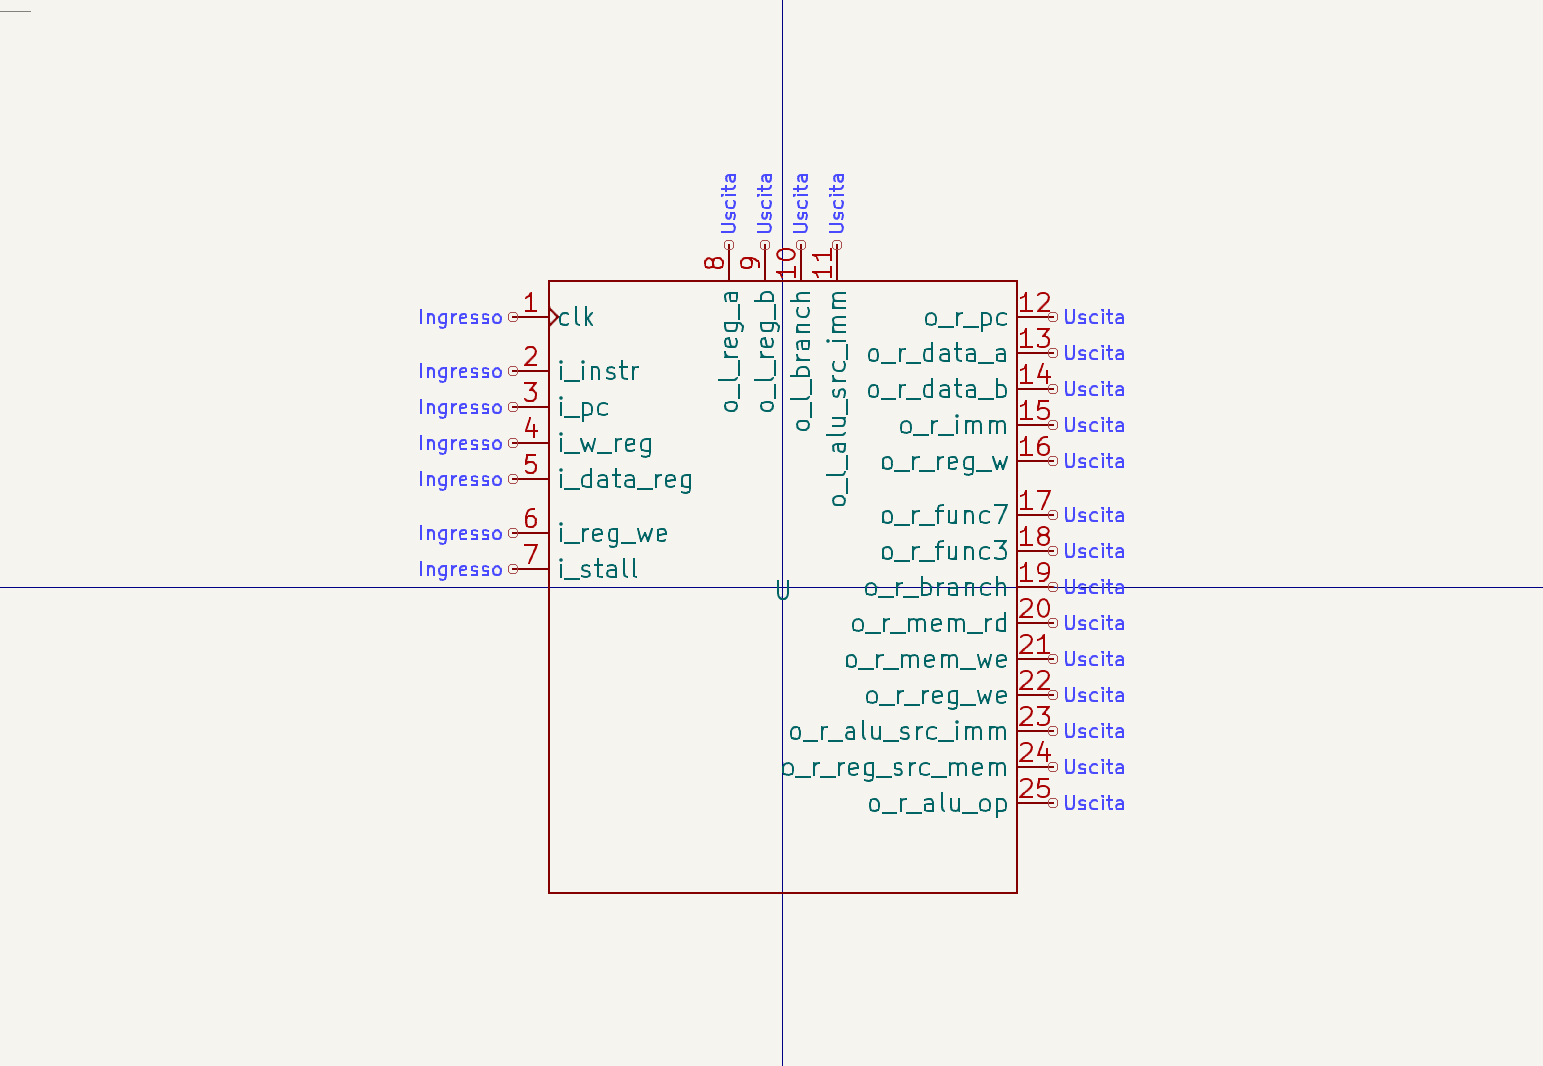
\includegraphics[width=0.9\textwidth,right,trim={400 150 400 150},clip]{components/Decode.png}
\end{minipage}

\subsection{Program counter}\label{PC}

    The \acrfull{pc} is a fundamental component in the Fetch stage of a pipelined \RISCV processor. 
    Its primary aim is to hold the address of the next instruction to be executed. 
    At the beginning of each instruction cycle, the Program Counter's value is used to fetch the instruction from memory. 
    Once the instruction is fetched, the \PC is incremented to point to the subsequent instruction in memory.
    
    The update might simply be an increment by a constant value, or it might involve more complex operations, 
    such as adding an offset for branch instructions. The ability to change the \PC value dynamically is crucial for 
    handling control flow changes, like jumps, branches, and subroutine calls, enabling the processor to execute instructions 
    out of sequential order when required.
    This increment is by a fixed amount, corresponding to the size of each instruction in the instruction set architecture \cite{chatgpt}.
    
    In my case my program \RAM provided 32-bit data, so the length of the instructions defined by the the \ISA themselves. 
    This is a difference with the pure \RISCV \ISA, so \textbf{my implementation is not completely compliant with \RISCV specifications}, 
    I choose to not conform totally because I had to adapt the code even if 
    I had used \RISCV specifications because the \gls{linking} process that concern with address calculations 
    is related to the memory layout that in our case is different to the standard one that usually is present in true computer.
    So in my case it every instruction is far away from the nearest by 1 memory location. 

    In my implementation it takes in input three signals:
    \begin{itemize}
        \item \texttt{stall},
            if asserted it should stop incrementing the \PC
        \item \texttt{branch taken},
            if asserted it means that the normal flow is interrupted and the \acrlong{pc} must take a specific value, 
            not the last number incremented (as the default behavior should be)
        \item \texttt{next instruction},
            this is the custom value that the \PC must take if the normal flow is interrupted
    \end{itemize}
    and in output it determines two signals. They both represent the current value of the \PC, but one it is stored in a register 
    the other is in input to the program memory \reff{P_MEM}, this is useful because every step takes a \gls{clk}, 
    and with the value stored it can calculate the new address during normal execution and 
    transmit its value to the Decode phase \reff{DECODE} in sync with the instruction to execute.

    My \PC have the register initialized to \texttt{0xFFFFFFFFFFFFFFFF} so that this number is summed 
    to the increment and (in my case is \texttt{0x0000000000000001}) the first instruction fetched 
    will be the one placed at memory address \texttt{0x0000000000000000}.

\subsection{Program memory}\label{P_MEM}
The program memory in a 5-stage pipelined \RISCV processor primary aim is to store the instructions that the processor will execute. 
This memory is distinct from the data memory \reff{D_MEM}, which holds the data operands and results of instructions. 
The program memory is typically implemented as a read-only memory (\ROM) or a non-volatile memory that retains 
the stored instructions even when the power is off, though it can also be implemented using \RAM in certain designs.

In the Fetch stage, the program memory works closely with the program counter (\PC), 
which keeps track of the address of the next instruction to be executed. 
The Fetch stage retrieves or "fetches" the instruction stored at the address specified by the program counter. 
This involves the program counter sending the address to the program memory, which then outputs the instruction located at that address. 
This fetched instruction is then passed on to the next stage in the pipeline for decoding and execution \cite{chatgpt}.

In my case my memory took in input only the address to read and is read-only (so a \ROM). 
It takes in input 64-bit input and provide 32-bit data (the instructions). 
It is a \SI{1}{KiB} memory, so the address can assume values $\in [\texttt{0x00}:\texttt{0xFF}]$, 
if it is more than the maximum, it saturates the value to \texttt{0xFF} and return the data located at this very last valid address.
    
\subsection*{Composition}

The fetch stage is composed by these two components and so takes in input the signals that determines 
the value of the \PC as described in \ref{PC}. After a \gls{clk} it provides the instruction and his associated address. 
The memory is linked with the \PC before its value is placed in the associated register, so that the \ROM 
can provide the instruction in sync with the \PC.


\section{Decode}\label{DECODE}
\begin{minipage}{0.48\textwidth}
This stage is responsible for interpreting the instruction and assert the right \glspl{control_sig} 
to choose the operation to perform on the data and his flow in and out the registers and the data memory.
Another important thing that happens during this stage is the reading of the register 
of the \textbf{register file} \reff{regfile}. The data is then forwarded to the following stage.
\end{minipage}
\begin{minipage}{0.48\textwidth}
  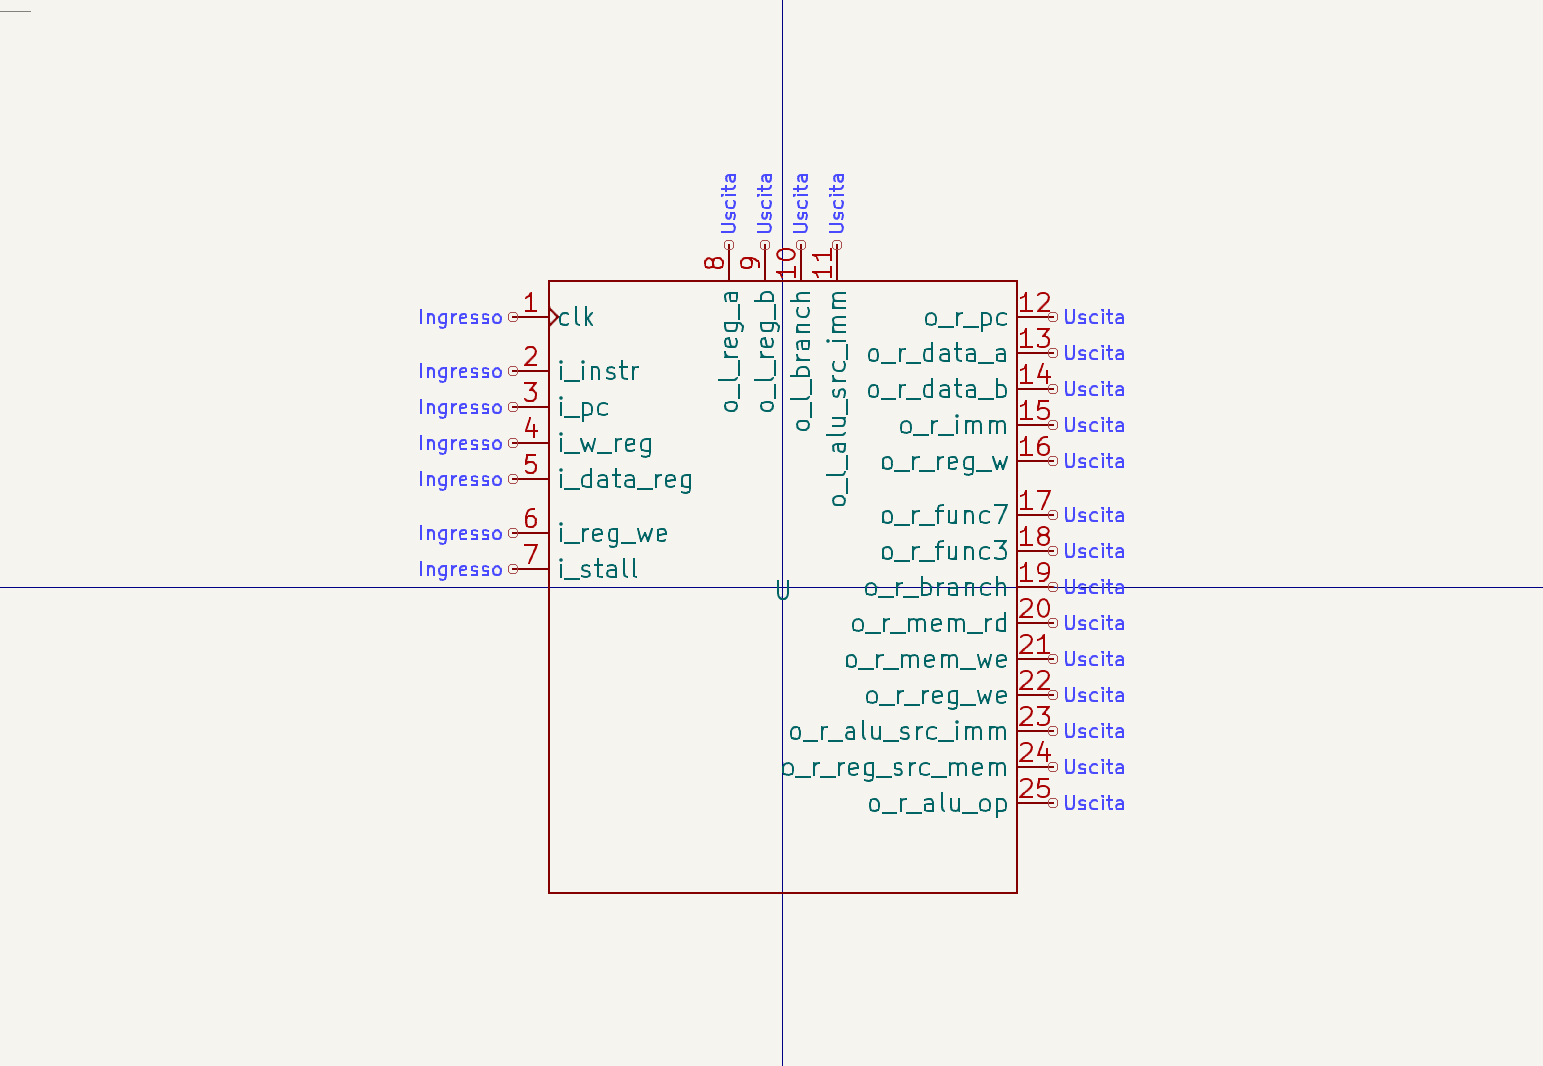
\includegraphics[width=0.9\textwidth,right,trim={400 150 400 150},clip]{components/Decode.png}
\end{minipage}

The control lines that are asserted are:
\begin{itemize}
    \item \texttt{branch}, this line is asserted if the instruction is a \emph{branch instruction} 
    (that can modify the program flow) for example \texttt{beq}
    \item \texttt{memory write}, this line is asserted if the data memory has to be written (\texttt{sd})
    \item \texttt{memory read}, this line is asserted if the data memory has to be read (\texttt{ld})
    \item \texttt{register write}, this line is asserted if the register has to be written, for example \texttt{addi}
    \item \texttt{ALU source}, this line is asserted if the source of the second operand 
    to the \ALU has to be the immediate calculated by the immediate generator \reff{immgen} 
    (like in the case of \texttt{addi}) or a selected register (like in the case of \texttt{add})
    \item \texttt{register source}, this line is asserted if the register has to be overwritten 
    and the source of his new value has to be the data memory (\texttt{ld}). 
    If it is not asserted the source of the value has to be the result of the \ALU calculation (for example like in \texttt{add})
    \item \texttt{ALU operation}, \texttt{func7} and \texttt{func3} are forwarded 
    to the \textbf{\ALU control unit} \reff{ALU_CU} that determine precisely the operation that the \ALU must perform on the data.
\end{itemize}

This step takes as input also the \texttt{stall} signal. If this signal is asserted the \glspl{control_sig} 
are forced to be inactive (in my case $=$`\texttt{0}') in this way the instruction that is decoded act like as a \texttt{nop}.

The data that is forwarded by this stage is
\begin{itemize}
    \item \texttt{pc}, this is the address of the instruction decoded. With this number in the following stage 
    is calculated the new address if there is a branch operation
    \item \texttt{data a}, this is the data that was stored in the first register decoded. 
    The index of the register is encoded in the instruction.
    \item \texttt{data b}, this is the data that was stored in the second register decoded. 
    The index of the register is encoded in some instructions
    \item \texttt{immediate}, this is a number extended by the immediate generator \reff{immgen} that is encoded in some instructions
    \item \texttt{register to write}, this is the index of the register that has to be overwritten
    \item \texttt{register a}, this is the register from which the first operand of the \ALU is taken. 
    This index is immediately forwarded to the \textbf{hazard detection unit} \reff{HDU} to check for any data \gls{hazard}
    \item \texttt{register b}, this is the same of the last but for the second register
\end{itemize}

\subsection{Register file}\label{regfile}
The register file in a \RISCV processor primary aim is to store and provide access to the processor's general-purpose registers, 
which are used to hold intermediate data and addresses during instruction execution.

The register file consists of an array of registers, typically 32 in the case of a standard \RISCV implementation, 
each capable of holding a fixed amount of data, such as 32 or 64 bits. 
When an instruction is fetched and decoded, the register file is accessed to retrieve 
the values stored in the source registers specified by the instruction. 
These values are needed for the execution of various operations, such as arithmetic computations, 
logical operations, and address calculations. In addition to reading data, the register file also supports writing data back to a register. 
This write operation occurs in the write-back stage \reff{WB} of the pipeline, 
where the result of an instruction is written back into a designated destination register \cite{chatgpt}.

My implementation deals only with 64-bit data, so every register of the 32 that are present, is 8-byte wide. 
As specified in the \ISA, the register with index 0 (\texttt{x0}) is hardwired to the value \texttt{0x0000000000000000}. 
This register file firstly read the data and then if is asserted the right pin, a register is overwritten.

\subsection{Control unit}
The control unit in a \RISCV processor plays a critical role in coordinating the operations of the processor 
by generating the necessary control signals based on the instruction being executed. 
Its primary aim is to interpret the fetched instruction and generate the appropriate signals to direct 
the activities of other components within the processor, ensuring that each instruction is executed correctly.

In the decode stage, the control unit reads the instruction, which contains the operation code (opcode). 
By analyzing this code, the control unit determines the nature of the operation to be performed, 
such as arithmetic, logic, memory access, or branch operations. 
Based on this determination, it generates control signals that guide the subsequent stages of the pipeline.

These control signals dictate the behavior of various parts of the processor, 
including the \acrfull{alu}, memory, register file, and multiplexers. 
For instance, the control unit will specify whether the \ALU should perform an addition or subtraction, 
whether data should be read from or written to memory, and which registers should be accessed for reading or writing data \cite{chatgpt}.

This is how I asserted the signals depending on the instructions:

\begin{center}
\begin{tabular}{|c|c|c|c|c|c|c|} 
\hline
 &\texttt{add} & \texttt{sd} & \texttt{ld} & \texttt{beq}, \texttt{bge} & \texttt{addi} & \texttt{nop} and unknown \\ 
 \hline
 \texttt{branch} & \xmark & \xmark & \xmark & \cmark & \xmark & \xmark \\ 
 \hline
 \texttt{memory read} & \xmark & \xmark & \cmark & \xmark & \xmark & \xmark \\
 \hline
 \texttt{memory write} & \xmark & \cmark & \xmark & \xmark & \xmark & \xmark\\
 \hline
 \texttt{register write} &\cmark & \xmark & \cmark & \xmark & \cmark & \xmark \\
 \hline
  \texttt{ALU source} &\xmark & \cmark & \cmark & \xmark & \cmark & \xmark \\
 \hline
  \texttt{register source} &\xmark & \xmark & \cmark & \xmark & \xmark & \xmark \\
 \hline
\end{tabular}
\end{center}


\subsection{Immediate generator}\label{immgen}
The aim of this component is to sign extend the immediate that is encoded in some instructions. 
This encoding for all the types that requires it and that I have implemented, 
specify the value with a 12-bit number, this immediate is than combined with the data in the register 
(for example to calculate an address for \texttt{ld} and \texttt{sd}) and must be a 64-bit number. 
For this reason this component enlarges the representation of the number according to his sign. 
To perform this operation it takes in input the whole instruction, it extracts the \texttt{opcode} and read the number accordingly.
\subsection*{Composition}
The Decode input takes the whole instruction and split his different fields. In particular, it takes the \texttt{opcode} 
and send it to the Immediate Generator Unit and to the Control Unit. The Control Unit set the right control signals if the \texttt{stall}
signal is not asserted. The Immediate Generator takes the same \texttt{opcode} and extracts the immediate of 12-bit, then sign-extend it.

\section{Execute}
\begin{minipage}{0.48\textwidth}
This stage is responsible for implementing the right operation on the right operands and so perform
the required calculation. It takes in input from the previous step the data from the two selected
registers (the second one will not be used for I-Type instructions). It takes the immediate that will be used
if the operation is not an R-Type instruction. In input there is also two other signals that for some instructions
complete the \texttt{opcode}; these are \texttt{func3} and \texttt{func7} that are forwarded to the 
ALU Control Unit \reff{ALU_CU}. This unit will set the right value to a signal that determine precisely
the operation that the \ALU will perform. In my case the \ALU can perform only additions and subtractions.
\end{minipage}
\begin{minipage}{0.48\textwidth}
  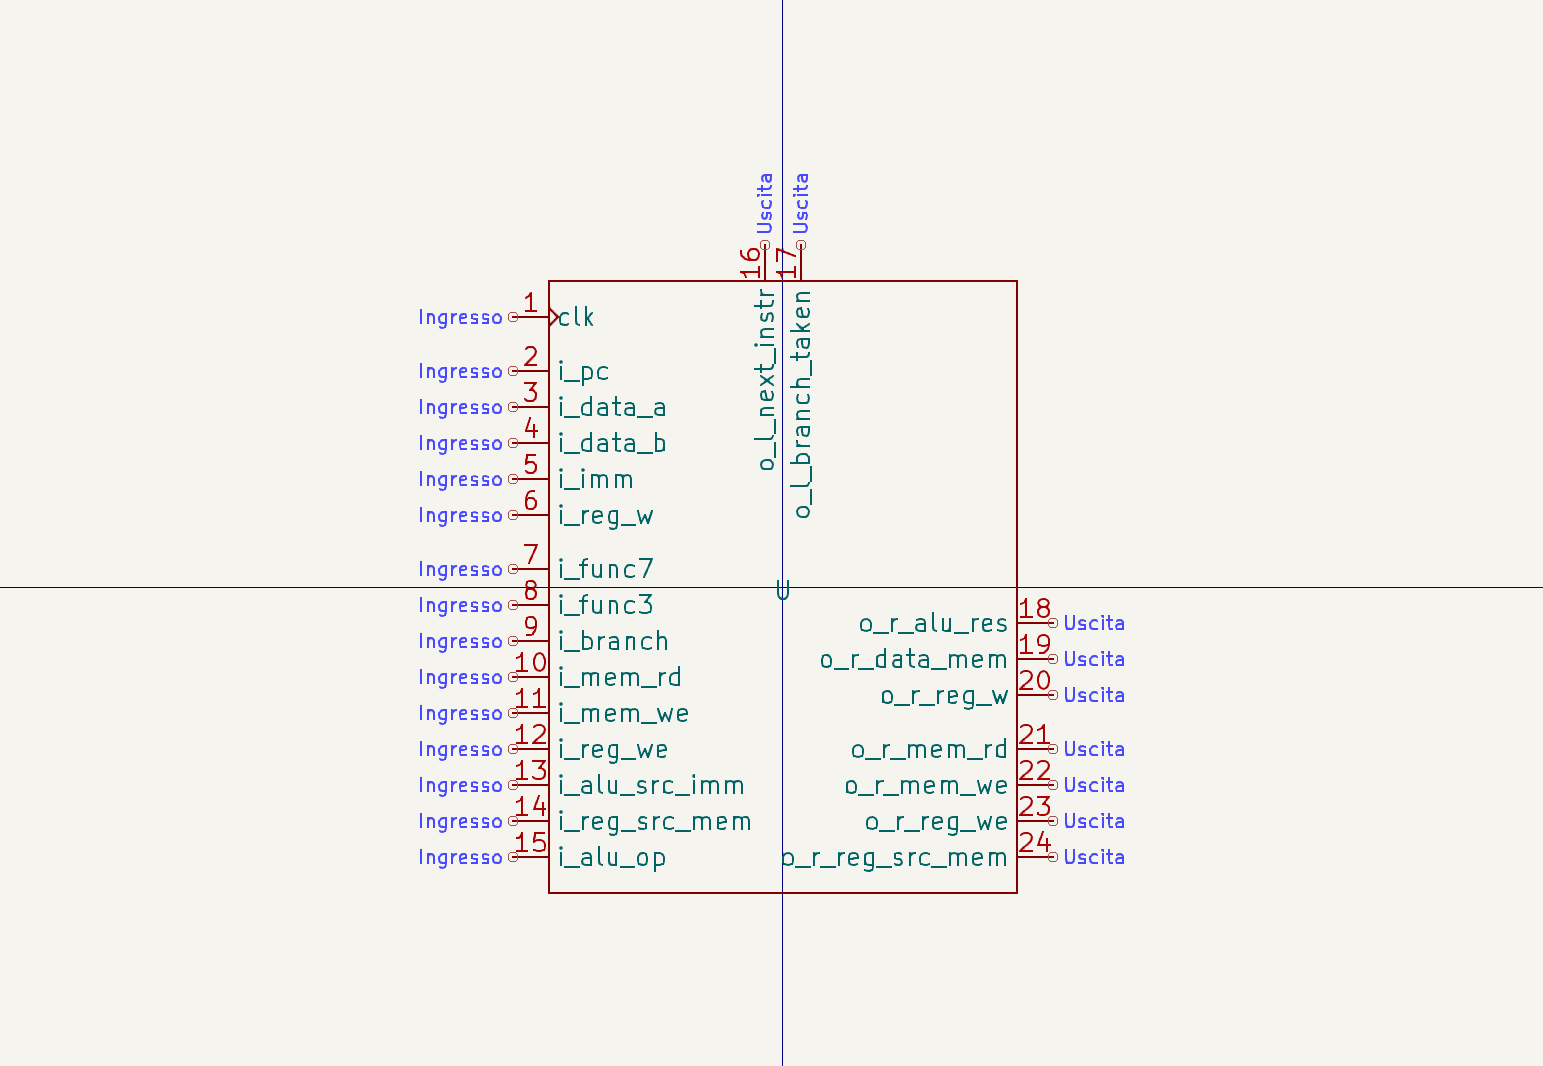
\includegraphics[width=0.8\textwidth,right,trim={400 150 400 150},clip]{components/Execute.png}
\end{minipage}

In this phase if the instruction is a branch instruction, the immediate is used for calculate
a new address from the current \PC using an independent full-adder. According to the \ISA, the value 
of the immediate must be shifted by 1 bit to permit only jump to address with the same parity
of the current address. In my implementation there is an $1:1$ relation between the addresses and 
the instructions; for this reason I choose to not conform to the \ISA and do not perform this shift.

The outputs are the result of the \ALU calculation, the data to store in the memory if the instruction is
\texttt{sd} (that in this case is taken from the second register specified), and the \glspl{control_sig}
that determine if the data memory has to be written or read and if a specific register has to be overwritten,
which it will be and if it will be overwritten with a data that was in memory or with the \ALU result.
 
\subsection{ALU}
This is the part of the processor that implement the calculation between the operands determined.
Usually this unit can support a wide variety of basic arithmetic operation like sums, subtractions,
shifts and logic operations like bitwise AND and bitwise OR of the operands. 

My implementation support only sum and subtraction. For performing this operation it uses a full-adder
implemented as described by the section \textbf{Full Adder} of the Wikipedia page 
\href{https://en.wikipedia.org/wiki/Adder_(electronics)}{Adder (eletronics)}. This adder takes in input
also a flag that determine if the operation is a true addition or if you want to add the second operand
in his negative representation (so perform a subtraction). To get the negative representation the 
operand is negated bitwise and is added summed a $+1$. This is easy to implement because in the standard
implementation the full-adder is a concatenation of 1 bit full adders that takes in input the previous
carry and the two bits and add them. They provide the result of the sum and the carry for the subsequent
adders. With this setup the carry of the first adder should be hardwired to `\texttt{0}', but it is
set to `\texttt{1}' if the operation is a subsection and to have the negative representation of the second
operand it is required to add the $+1$.

\subsection{ALU control unit} \label{ALU_CU}
This component takes in input the \texttt{func3} and \texttt{func7} fields and set the right 
\texttt{ALU operation} code. In my implementation it uses also the \texttt{func3} field to
distinguish the \texttt{beq} and \texttt{bge} instructions (that have the same \texttt{opcode}).

I choose to delegate this unit to distinguish between the two because I wanted the Control Unit
to only takes in input the \texttt{opcode}. With this idea in mind maybe the name 
`\textbf{ALU control unit}' it is not accurate, because it determines other characteristics other
than the operation to perform. 

\subsection*{Composition}
The data of the two register and the immediate are linked to the \ALU. A 1-bit \acrshort{mux} determines if
the immediate or the data from the second register must be used in the operation (this \acrshort{mux} is selected
by the \texttt{ALU source} signal in input).

The program counter is summed to the immediate by an independent adder. The result will be the
instruction address from which continue the execution if the instruction changes the normal
program flow and a branch is taken. If this last is taken a signal is asserted. This signal
will notify the \acrshort{hdu}.

All the results are stored in a register with the exception of the \texttt{branch taken} signal and 
the signal with the value of the next instruction to execute. This is because a branch is taken
at this stage of the pipeline, so there is no need to store the information and to forward it
to the next stages.


\section{Memory Access}
\begin{minipage}{0.48\textwidth}
This stage is responsible for reading the data memory if a \texttt{ld} instruction is executed, 
or to overwrite it with a \texttt{sd}. 
This stage takes in input the data to write to the memory, the \ALU result (that if the
instruction is a \texttt{ld} or a \texttt{sd} determine the location in memory to deal with)
and all the control signals related to the register to overwrite if the instruction imply it.


\end{minipage}
\begin{minipage}{0.48\textwidth}
  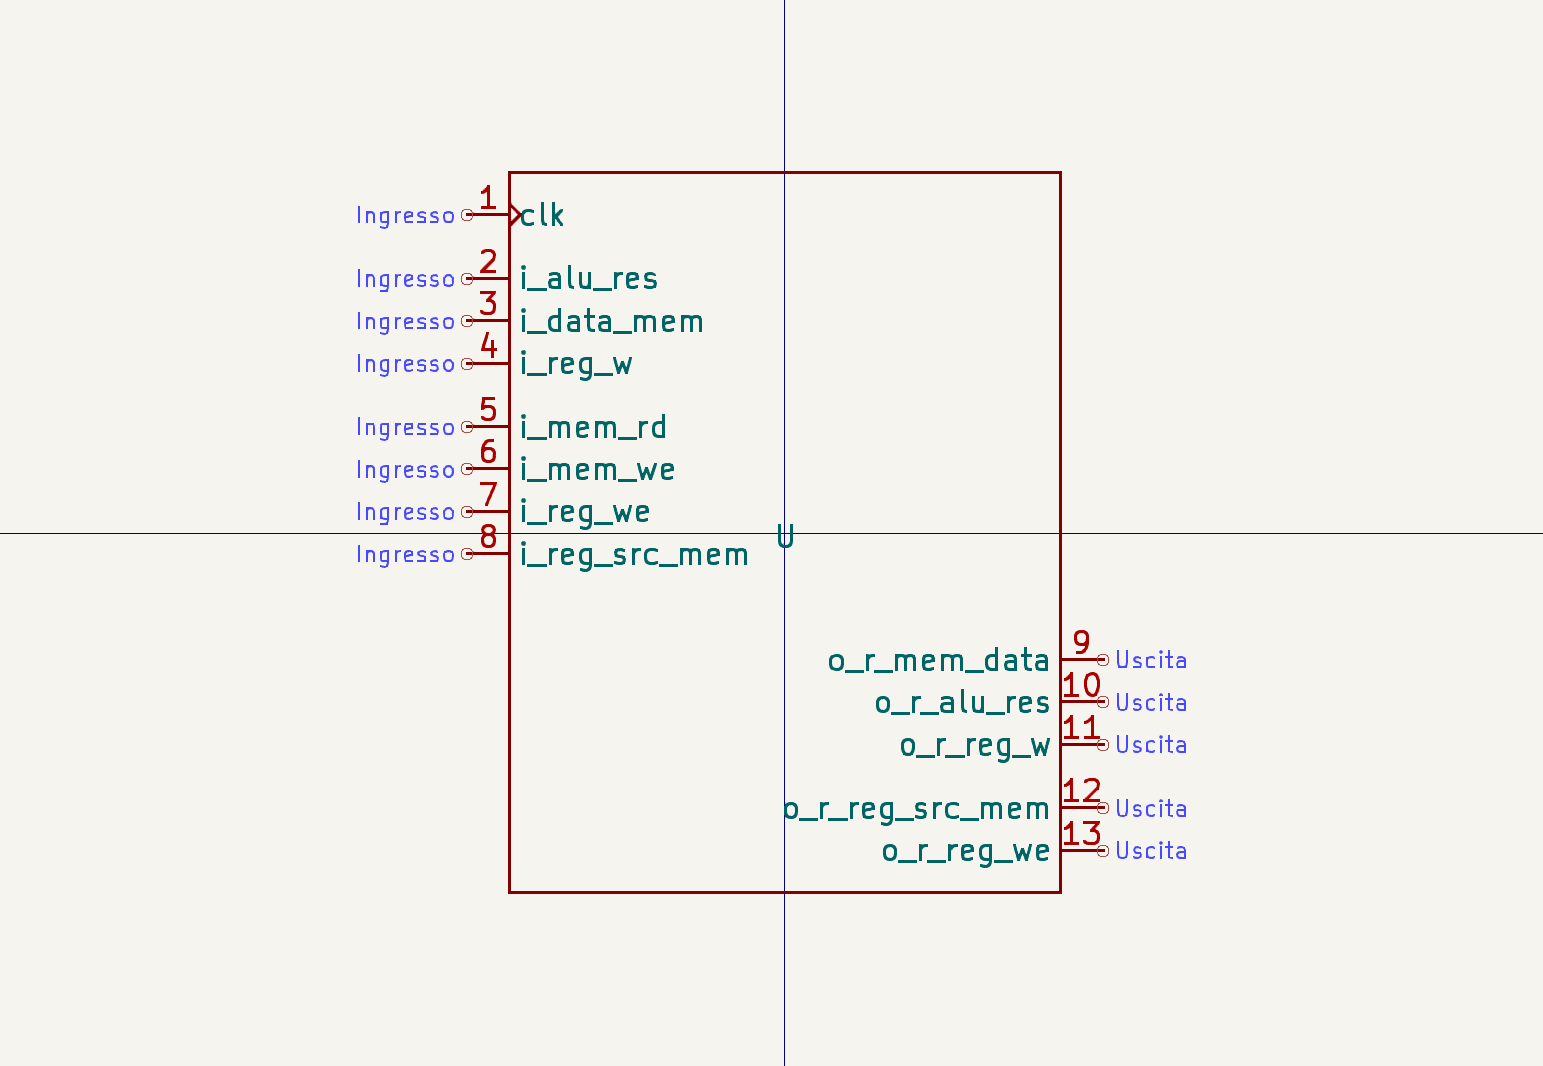
\includegraphics[width=0.7\textwidth,right,trim={350 150 350 150},clip]{components/MemoryAccess.png}
\end{minipage}

\subsection{Data memory}\label{D_MEM}
Every memory entry is initialized to \texttt{0x0000000000000000} (in my implementation the first 12 data
entry are initialized to an array that I want to sort with the \sort algorithm that I have hard coded on
the program \ROM).

The memory takes a \gls{clk} to be written or read and saturates the address as explained for the program memory \reff{P_MEM}
and support \SI{1}{KiB}.


\section{Write Back and top hierarchy processor}\label{WB}
Te Write Back stage is responsible for overwrite the register file that is placed inside the Decode entity.
I didn't implement a whole entity, because the logic that is needed is only a 1-bit \acrfull{mux} selected
by the \texttt{register source} \gls{control_sig} that if asserted overwrite the register file with data
read from the memory, otherwise with the \ALU result. I implemented this logic into the top hierarchy component \textbf{\acrshort{cpu}}.

\subsection{Hazard detection unit}\label{HDU}
\begin{minipage}{0.48\textwidth}
The last component that is present in the top hierarchy entity is the \acrfull{hdu} that is a component responsible for the detection
of control \glspl{hazard} and \glspl{hazard}. If it detects these \glspl{hazard}, it asserts the \textbf{stall} signals for the Fetch
and the Decode steps. Taking into account that these two different types of occurs requires a different management of the stalls,
the \acrshort{hdu} manage the two independently.

Let's analyze separately the two types of \gls{hazard}:
\end{minipage}
\begin{minipage}{0.48\textwidth}
  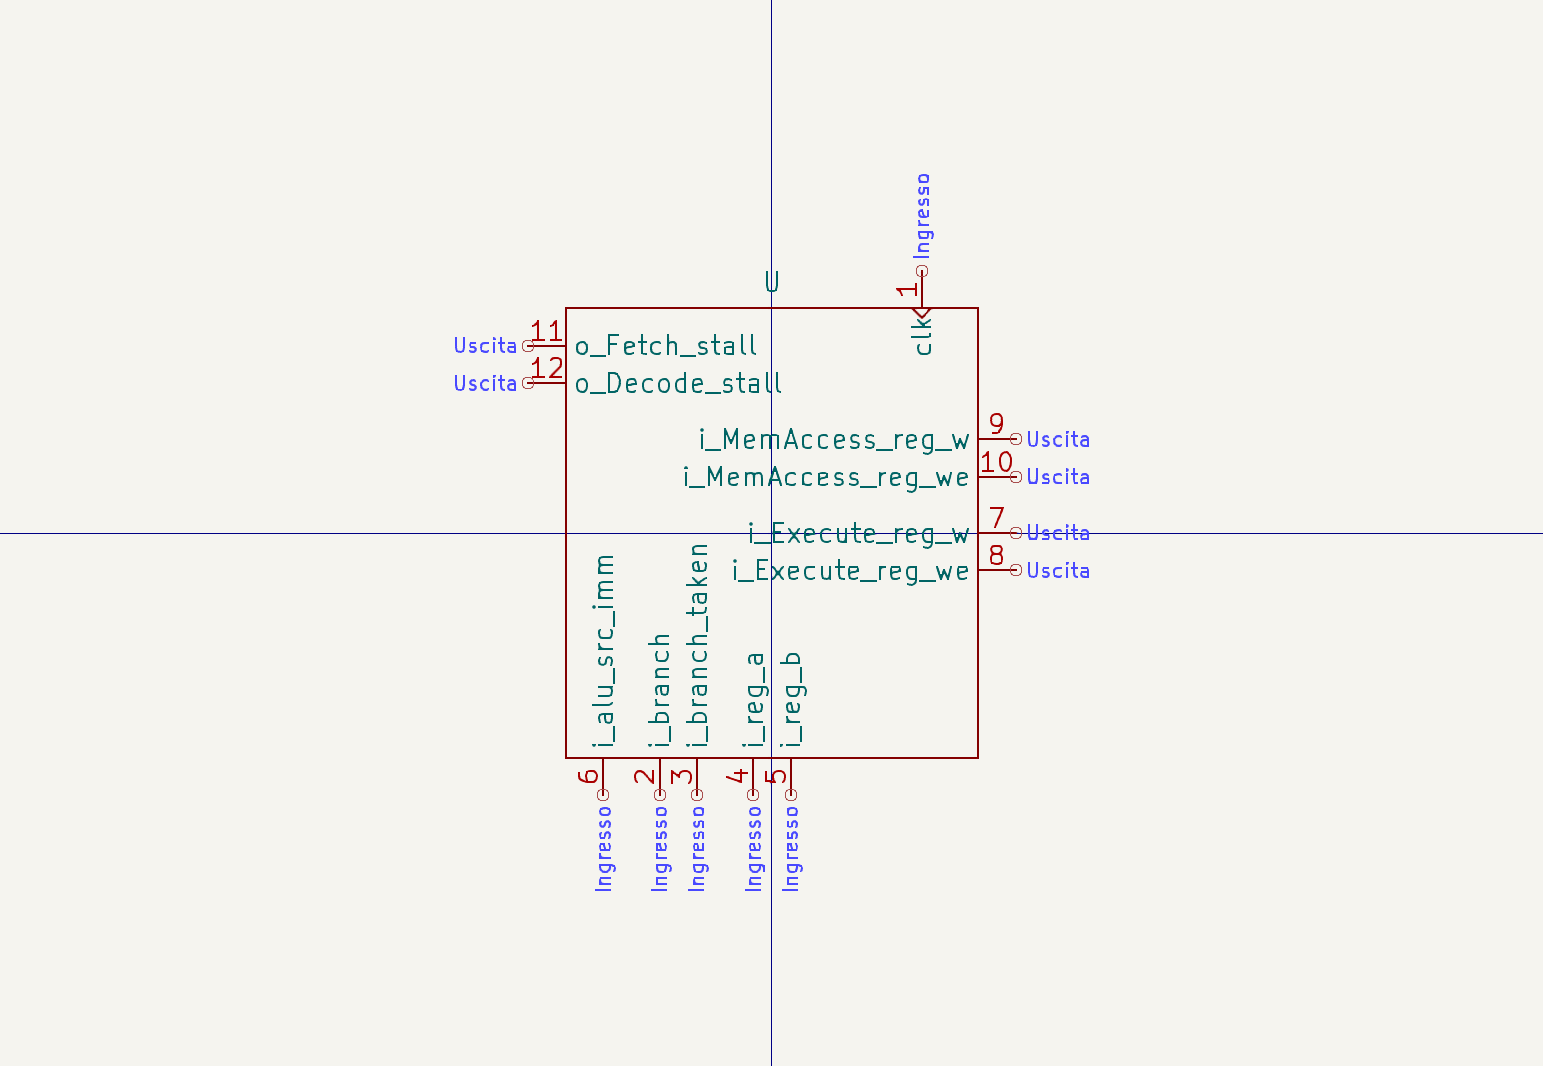
\includegraphics[width=0.7\textwidth,right,trim={450 150 450 150},clip]{components/HDU.png}
\end{minipage}
\subsubsection{Data hazard}
This type of \gls{hazard} take place if one of the registers used in the calculation by the current instruction is the same that
the register that have to be written by an earlier command that didn't finish his pipeline drive-through. In this case we want that
the processor stop the execution until the register is not overwrite and only then read that register and perform the following instruction.

It is possible to check which register an instruction requires in the Decode phase, before reading from the register file.
If an earlier instruction require to write a register means that the \texttt{register write enable} in the Execute phase
or in the Memory Access phase, will be asserted. If this is the case we want to \gls{stall} the Fetch to continue fetching 
the same instruction but also neutralize his effect until the register is written. To neutralize his effect we \gls{stall} the
Decode phase. We need a register in the \acrshort{hdu} because we have to wait a clock cycle after the \gls{hazard} is present
to have the time to complete the Write Back stage.
\subsubsection{Control hazard}
This type of \gls{hazard} take place if a branch instruction occurs. In this case we want to wait until we don't know the \ALU
result that determine if the branch is taken. If it isn't, we want to continue the execution, if it is, we want to neutralize
the effect of the next instruction until we did the jump and the correct instruction is fetched.

This means that to check if a control \gls{hazard} occurs we have to check only the type of the instruction right after the instruction
is decoded. A difference with the previous hazard is that we don't have to wait that an earlier instruction complete his pipeline, so we
\gls{stall} for a fixed amount of \glspl{clk} (in my implementation 1 is sufficient), so we use a register to determine when the \gls{stall}occurred.
During the \gls{stall} we have to neutralize the effect of the branch instruction itself to not \gls{stall} forever, and lastly we have to 
\gls{stall} for one more \gls{clk} the Decode phase if the branch is taken because we don't want to execute the instruction that follows the branch,
but we fetched it during the Execution step in which we calculate also the value of the next instruction.

\subsection*{Composition}
Finally, I connected the subsequent steps. The Decode and Execute steps and also connected to the \acrshort{hdu} as explained in \ref{HDU}.
The Write Back step consists in the connection between the Memory Access step and the register file in the Decode. 
Lastly the Execute after calculating the new instruction in case of a taken branch forward it to the Fetch phase.
The \acrshort{hdu} is connected to Fetch and Decode to \gls{stall} them.

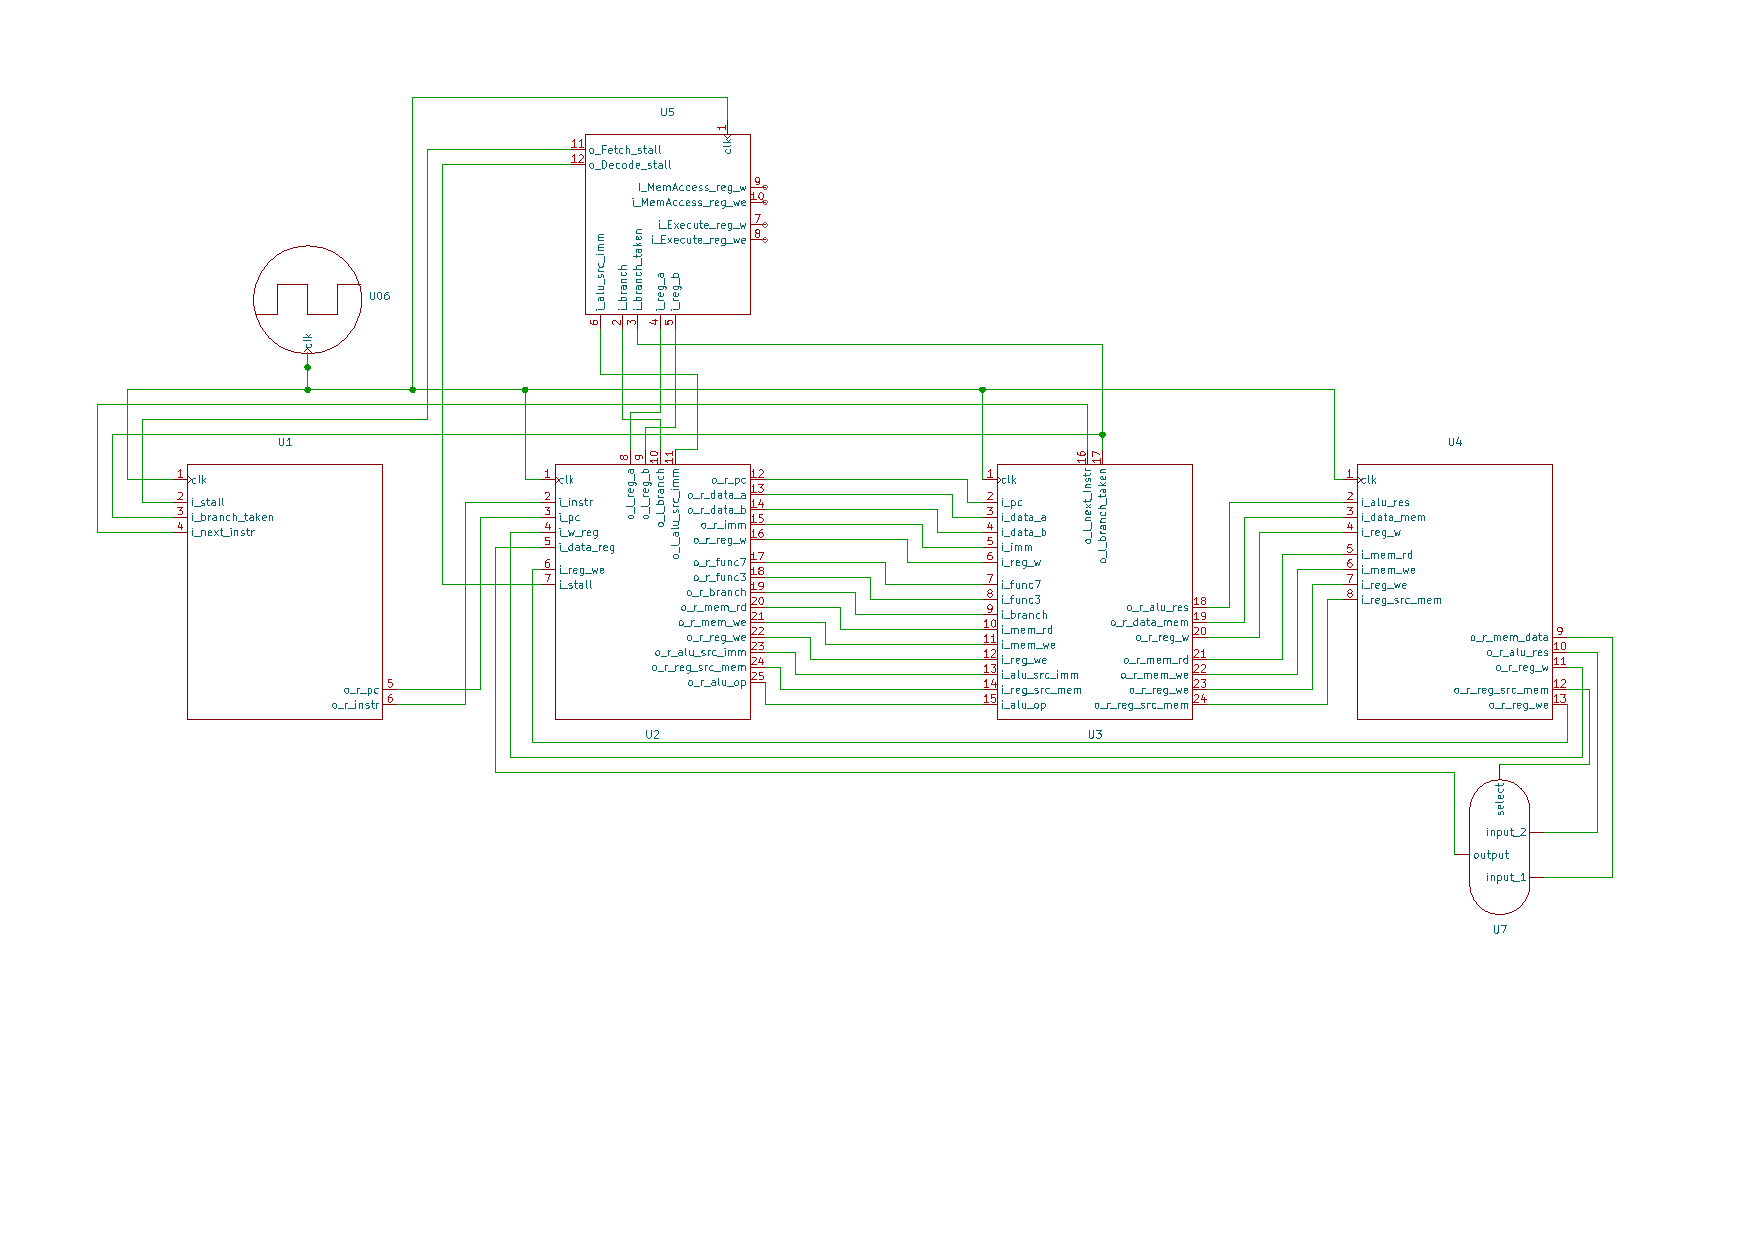
\includepdf[angle=90,pages=-]{components/processor}

\section{Conclusion}
I firstly programmed in \texttt{C} the \sort, then I cross-compiled it for \RISCV. After that looked at the assembly code, I tried to simplify
the instructions used and hard coded the new program translated in machine code into the program \ROM. I initialized the data ram with an array
and I simulated the functional behavior of the processor. I also added some instruction to load the data of the array in the data ram into the
\texttt{x0} register at the beginning and end of the \sort, so that analyzing the data of the \texttt{data to write on register} signal I would
see the unsorted array and [hopefully] the sorted one at the end. The simulation of the circuit was possible thanks to the 
\href{http://ghdl.free.fr/}{ghdl} software, and the wave visualization with \href{https://gtkwave.sourceforge.net/}{GTKWave}. 
I include the screenshot of the signal before and after the bubble sort:
\begin{center}
  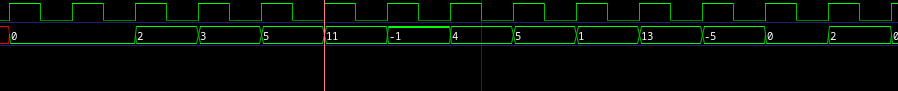
\includegraphics[width=\textwidth,trim={0 30 0 0},clip]{inputarray.png}
  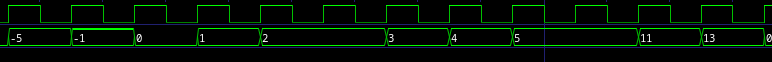
\includegraphics[width=\textwidth,trim={0 5 0 0},clip]{outputarray.png}
\end{center}


\section{Appendix}\label{prompts}
To retrieve this answers from \texttt{Chat GPT} I didn't provide more context than the one present in the prompts. 
I used clean and independent chat stateless sessions.
\subsection{Prompt and reply to describe the PC}\label{prompt:pc}
\begin{itshape}
    I am doing a project for which I am implementing a 5 stage pipelined RISCV processor in VHDL, my first step is the Fetch step. 
    In this step there is the Program Counter. 
    Can you describe the aim and the general functioning of a Program Counter just using text, no code and no lists? 
    I have to add it to the report that I am writing.
\end{itshape}

\begin{spverbatim}
The Program Counter (PC) is a fundamental component in the Fetch 
stage of a pipelined RISCV processor. 
Its primary aim is to hold the address of the next instruction to be executed. 
At the beginning of each instruction cycle, the Program Counter's value is used 
to fetch the instruction from memory. 
Once the instruction is fetched, the PC is typically incremented to point 
to the subsequent instruction in memory. 
This increment is usually by a fixed amount, 
corresponding to the size of each instruction 
in the instruction set architecture.

In more detail, during the Fetch stage, the PC's current value is sent to memory 
to retrieve the instruction located at that address. 
After this, the PC is updated to reflect the address of the next instruction. 
This update might simply be an increment by a constant value, 
or it might involve more complex operations, 
such as adding an offset for branch instructions. 
The ability to change the PC value dynamically 
is crucial for handling control flow changes, 
like jumps, branches, and subroutine calls, 
enabling the processor to execute instructions 
out of sequential order when required.

The PC operates in a cycle, ensuring a continuous flow of instruction addresses, 
which drives the overall execution process of the processor. 
Its design ensures that the processor can systematically and efficiently 
fetch and execute a sequence of instructions, 
while also providing flexibility for complex control 
flows in the program execution.
\end{spverbatim}


\subsection{Prompt and reply to describe the program memory}\label{prompt:pmem}
\begin{itshape}
I am doing a project for which I am implementing a 5 stage pipelined RISCV processor in VHDL, my
first step is the Fetch step. In this step there is the Program Memory (different from the data memory). 
Can you describe the aim and the general functioning of a program memory just using text, 
no code and no lists? I have to add it to the report that I am writing.
\end{itshape}

\begin{spverbatim}
The program memory in a 5-stage pipelined RISC-V 
processor serves a critical role in the Fetch stage, 
where its primary aim is to store the instructions that the processor will execute. 
This memory is distinct from the data memory, 
which holds the data operands and results of instructions. 
The program memory is typically implemented as a read-only memory (ROM) 
or a non-volatile memory that retains 
the stored instructions even when the power is off,
though it can also be implemented using RAM 
in certain designs for flexibility during development.

In the Fetch stage, the program memory 
works closely with the program counter (PC), 
which keeps track of the address of the next instruction to be executed. 
The Fetch stage retrieves or "fetches" the instruction stored 
at the address specified by the program counter. 
This involves the program counter sending the address to the program memory, 
which then outputs the instruction located at that address. 
This fetched instruction is then passed on to the next stage 
in the pipeline for decoding and execution.

The efficiency and speed of the program memory are crucial, 
as the Fetch stage sets the pace for the entire instruction execution pipeline. 
If the program memory access is slow, it can create bottlenecks 
that degrade the overall performance of the processor. 
To mitigate this, program memories are often designed with fast access times and 
may utilize caching mechanisms to further enhance performance.

Overall, the program memory's functionality is foundational 
to the operation of a pipelined processor, 
ensuring that instructions are promptly and accurately fetched, 
allowing for smooth and efficient instruction 
execution throughout the pipeline stages.
\end{spverbatim}


\subsection{Prompt and reply to describe the register file}\label{prompt:regfile}
\begin{itshape}
I am doing a project for which I am implementing a 5 stage pipelined RISCV processor in VHDL, 
my second step is the Decode step. In this step there is the Register File. Can you describe the aim and
the general functioning of a register file just using text, no code and no lists? I have to add it to
the report that I am writing.
\end{itshape}

\begin{spverbatim}
The register file in a RISC-V processor is a crucial 
component within the decode stage of the pipeline. 
Its primary aim is to store and provide rapid access 
to the processor's general-purpose registers, 
which are used to hold intermediate data and addresses during instruction execution.

The register file consists of an array of registers, 
typically 32 in the case of a standard RISC-V implementation, 
each capable of holding a fixed amount of data, such as 32 or 64 bits. 
When an instruction is fetched and decoded, the register file is accessed 
to retrieve the values stored in the source registers specified by the instruction. 
This step is essential because these values are needed 
for the execution of various operations, such as arithmetic computations, 
logical operations, and address calculations.

During the decode stage, the instruction is examined 
to determine which registers are being referenced. 
The register file then reads the values from the specified 
source registers and makes them available for the subsequent execution stage. 
In addition to reading data, the register file 
also supports writing data back to a register. 
This writes operation typically occurs in the write-back stage of the pipeline, 
where the result of an instruction is written back 
into a designated destination register.

The register file is designed for fast access 
to support the high-speed requirements of the pipeline. 
It achieves this by using dual read ports and one write port, 
allowing two registers to be read simultaneously 
and one register to be written at the same time, 
which is a common requirement for most instructions. 
This parallelism is essential for maintaining 
the efficiency and throughput of the pipelined processor.

In summary, the register file serves as a high-speed storage and 
retrieval unit for the processor's registers, 
playing a vital role in ensuring that the necessary data is readily 
available for each instruction as it progresses through the pipeline. 
Its efficient design is fundamental to achieving 
the overall performance goals of the processor.
\end{spverbatim}


\subsection{Prompt and reply to describe the control unit}\label{prompt:cu}

\begin{itshape}
I am doing a project for which I am implementing a 5 stage pipelined RISCV processor in VHDL, 
my second step is the Decode step. In this step there is the Control Unit. Can you describe the aim and
the general functioning of a control unit just using text, no code and no lists? I have to add it to
the report that I am writing.
\end{itshape}

\begin{spverbatim}
The control unit in a RISC-V processor plays a 
critical role in coordinating the operations 
of the processor by generating the necessary 
control signals based on the instruction being executed. 
Its primary aim is to interpret the fetched 
instruction and generate the appropriate signals 
to direct the activities of other components within the processor, 
ensuring that each instruction is executed correctly and efficiently.

In the decode stage, the control unit 
reads the instruction, which contains the operation 
code (opcode) and, in some cases, additional function codes. 
By analyzing these codes, the control unit determines the nature 
of the operation to be performed, such as arithmetic, 
logic, memory access, or branch operations. 
Based on this determination, it generates control signals 
that guide the subsequent stages of the pipeline.

These control signals dictate the behavior of various parts of the processor, 
including the arithmetic logic unit (ALU), memory, register file, and multiplexers. 
For instance, the control unit will specify 
whether the ALU should perform an addition or subtraction, 
whether data should be read from or written to memory, 
and which registers should be accessed for reading or writing data.

The control unit ensures that the correct data paths are selected, 
enabling the processor to handle different 
types of instructions in a streamlined manner. 
It orchestrates the timing of operations, managing the flow 
of data through the pipeline stages to prevent conflicts and 
ensure that each instruction progresses 
smoothly from fetch to execution to write-back.

In summary, the control unit is essential for decoding instructions 
and generating the necessary control signals to manage the processor's operations, 
enabling the processor to execute a wide variety 
of instructions efficiently and accurately.
\end{spverbatim}

\clearpage
\printglossary
\clearpage



\nocite{*}
\bibliographystyle{alpha}
\bibliography{utils/bibliography}


\end{document}